\documentclass[10pt,conference,compsocconf]{IEEEtran}

%\usepackage{times}
%\usepackage{balance}
\usepackage{amsmath}
\usepackage{url}
\usepackage{graphicx}
\usepackage[pdftex]{hyperref}
\usepackage[utf8]{inputenc}

\usepackage{tikz}
\usetikzlibrary{shapes,arrows}

\begin{document}
\title{Inpainting with controlled dimensionality reduction in the Fourier domain}

\author{
  Group: NoobzRockz\\
  Patrick Bänziger, Kaspar Etter, Jan Rüegg\\
  Department of Computer Science, ETH Zurich, Switzerland
}

\maketitle

\begin{abstract}
The abstract should really be written last, along with the title of
the paper. The four points that should be covered~\cite{jones08}:
\begin{enumerate}
\item State the problem.
\item Say why it is an interesting problem.
\item Say what your solution achieves. (CLAIM!)
\item Say what follows from your solution.
\end{enumerate}
\end{abstract}

\section{Introduction}
Inpainting is about reconstructing the missing spots of an image by guessing the correct values. The quality of such a restoration method can be evaluated by masking an image and comparing the result with the original.\\
Our approach is based on the assumption that (natural) images have some underlying characteristic that can be distinguished from noise. The computed pixels can be viewed as a disturbed version of the genuine ones, hence the goal is to get rid of this noise. We do so by analyzing image patches in the Fourier space, removing the weak frequencies that (hopefully) capture the noise and thereby recovering the intrinsic signal.\\
We repeat this procedure with the newly determined values until the error of a randomly chosen validation set converges or the maximum number of iterations is reached. For a faster start, we initialize our reconstructed image with what we call Gaussian interpolation: Using MATLAB's filtering function, we compute a weighted sum over all the neighboring pixels that are known. In order to determine the best threshold for suppressing weaker frequencies, we randomly remove even more pixels from the image and use them as a validation set (for which we know the correct values).

\section{Methods}
\subsection{Related work}
Without actually knowing the broad field of research about inpainting (also known as image interpolation), we could not find any papers covering similar concepts as ours. Most methods are based on partial differential equations or some form of texture synthesis.

\subsection{New approach}

% Define block styles
\tikzstyle{decision} = [diamond, draw, fill=blue!20, 
    text width=4.5em, text badly centered, inner sep=0pt]

\tikzstyle{block} = [rectangle, draw, fill=blue!20, 
    text width=7em, text centered, rounded corners, minimum height=4em]

\tikzstyle{line} = [draw, -latex']

\tikzstyle{cloud} = [draw, ellipse,fill=red!20,
    minimum height=2em]
    
\begin{figure}
\begin{tikzpicture}[node distance = 2cm, auto]
  % Place nodes
  \node [cloud] (node1) {Start};
  \node [block, right of=node1, node distance = 3.1cm] (node2) {Remove validation set};
  \node [block, below of=node2] (node3) {Frame image};
  \node [block, below of=node3] (node4) {Gaussian interpolation};
  \node [decision, below of=node4] (node5) {Iterative?};
  \node [block, right of=node5, node distance = 3.1cm, fill=green!20] (node6) {Find best threshold};
  \node [block, below of=node6, fill=green!20] (node7) {Reset known values except validation set};

  \node [block, left of=node5, node distance = 3.1cm] (node8) {Find best threshold};
  \node [block, below of=node8] (node9) {Gaussian interpolation on original data};
  \node [block, below of=node9] (node10) {Apply best threshold};

  \node [block, right of=node10, node distance = 3.1cm] (node11) {Unframe image};
  \node [block, below of=node11] (node12) {Reset known values};
  \node [cloud, right of=node12, node distance = 3.1cm] (node13) {End};

  % Draw edges
  \path [line] (node1) -- (node2);
  \path [line] (node2) -- (node3);
  \path [line] (node3) -- (node4);
  \path [line] (node4) -- (node5);
  \path [line] (node5) -- node[above]{yes} (node6);
  \path [line] (node5) -- node[above]{no} (node8);

  \draw [->] (node6) to [bend left=20] (node7);
  \draw [->] (node7) to [bend left=20] (node6);

  \path [line] (node8) -- (node9);
  \path [line] (node9) -- (node10);
  \path [line] (node10) -- (node11);
  \path [line] (node11) -- (node12);
  \path [line] (node12) -- (node13);

  \path [line] (node7) |- (node11);
\end{tikzpicture}
\caption{Our newly proposed algorithm as a flowchart.}
\label{flowchart}
\end{figure}

As outlined in the introduction, we combined several ideas for obtaining an inpainting algorithm that provides both good results and fast performance. The input of our algorithm is the image to be restored together with a mask that indicates its unknown spots.\\
Before entering the iterative part of our algorithm, the following three steps are performed (as seen in figure \ref{flowchart}):
\begin{enumerate}
\item In order to guide the elimination of frequencies by finding the optimal threshold (as described below), we first remove additional pixels from the image and use them as the validation set. The fraction of additional pixels to be removed is a global parameter, which we optimized using gradient descent (as explained in section \ref{gradient_descent}).
\item Since our reduction in the Fourier space works best with framed patches, we frame the complete image by mirroring its margin. (The size of the frame is another optimizable global parameter.)
\item For obtaining an initial reconstruction of the image, we compute a weighted sum over all the neighboring pixels that are known. By setting all unknown pixels in the image to zero and encoding known values with 1s in the mask, elementwise division of the filtered image by the similarly filtered mask results in a normalized sum weighted by the filtering kernel. (This procedure, which we call Gaussian interpolation, allows us to use MATLAB's fast native functions and to fill holes up to the kernel size, which is another global parameter.)
\end{enumerate}

After these preparing steps, we start to iteratively improve the reconstructed image with the following steps:
\begin{enumerate}
\item Using the abovementioned validation set, we evaluate several thresholds for every patch and keep for each the best one: After calculating a fast Fourier transform for every patch, frequencies weaker then the threshold are suppressed by setting them to 0. Since profiling showed that the Fourier transform with its inverse is by far the most time-consuming part of our algorithm, we try to perform as few threshold evaluations as possible. For this purpose, we iteratively evaluate two new thresholds around a center threshold, taking the best one as the new center and decreasing the offset. For this optimization as well as for the whole iteration, we have both a number- and a convergence-based termination criterion.
\item Having stored the reconstruction of every patch with its best threshold, all that remains to do is copying the newly estimated missing pixels (including those of the validation set) back into the reconstructed image.
\end{enumerate}
Finally, the frame added in the beginning is removed again and the pixels of the validation set are overwritten by the original ones. A variant of the presented method is to do it non-iteratively and revert to the original data after determining the thresholds, such that the Gaussian interpolation and the thresholding in the Fourier space is performed without the validation set.

\subsection{Global parameter optimization}
\subsubsection{Optimized parameters}
As shown in table \ref{parameters}, our algorithm has a total of 10 parameters that can be set globally. Instead of tuning them by hand, we automated the optimization process and implicitly use the best parameters found so far, which we store in the file system. This feature also allows us to interrupt the optimization process at any time and continue with the best parameters later on.

\begin{table*}
\begin{center}
\begin{tabular}{|l|l|r|r|}
\hline
Parameter & Description & Initial value & Optimized value\\
\hline
gauss\_size & Size of the Gaussian kernel & ? & ? \\
gauss\_sigma & Sigma of the Gaussian kernel & ? & ? \\
patch\_size & Patch size as exponent to the basis 2 & ? & ? \\
patch\_frame\_size & Frame size in pixels & ? & ? \\
td\_abortbelow\_stdev & Minimal standard deviation while evaluating thresholds & ? & ? \\
td\_abortbelow\_stepsize & Minimal step size while evaluating thresholds & ? & ? \\
td\_middle & Initial threshold & ? & ? \\
validation & Fraction of pixels in the validation set & ? & ? \\
max\_iterations & Maximum number of iterations & ? & ? \\
abortbelow\_change & Minimal change for performing another iteration & ? & ? \\
\hline
\end{tabular}
\end{center}
\caption{Parameters with their initial and optimized values.}
\label{parameters}
\end{table*}

\subsubsection{Gradient descent}
\label{gradient_descent}
We optimize all parameters at once using a method called gradient descent. Since our cost function is based on measurements, we cannot derive it with respect to individual parameters and have to determine the gradient with finite differences. Besides weighting the parameters with respect to their improvements (which gives us the slope), we also defined a momentum term that should help us to overcome local minima.

\subsubsection{Cost function}
For optimizing a set of parameters, a cost function is needed. Its most important component is obviously the error function used in the submission system, which calculates the mean over the squared differences between the reconstructed and the original image. However, without including the performance of the algorithm, the runtime could grow arbitrarily to get the best accuracy possible. We considered several cost functions based on the error $E$ and the time $T$ (see table \ref{error_functions}). These two values are scaled appropriately: Usually, the error is multiplied by a factor of 10'000 and the time (measured in seconds) by a factor of 0.01.

\begin{table*}
\centering
\begin{tabular}{|l|p{6cm}|p{6cm}|}
\hline
Function & Advantages & Disadvantages \\
\hline
$E + T$ & Easy to understand and everywhere a good gradient & Linear improvement does not necessarily follow one's intuition about the ordering of results \\
\hline
$\exp(E)+\exp(T)$ & Fast increase for both error and time & Not enough gradient for very low $E$ and $T$ values \\
\hline
$(1-\exp(E))*(1-\exp(T))$ & Allows very large times for very low errors & Also true vice versa, i.e. a minimization in time \\
\hline
$\begin{cases}
E & \text{if }T<60\\
E+\exp(T/60 - 1) - 1 & \text{otherwise}
\end{cases}$ & Continuous function that optimizes for error only when the time is below a certain value but penalizes long times. & Seems to work quite well and therefore used by us \\
\hline
\end{tabular}
\caption{Various cost functions used in the optimization process.}
\label{error_functions}
\end{table*}

\subsubsection{Sample data}
We used the three images provided for the last exercise (consisting of both natural and artificial images) to evaluate the accuracy and performance of the chosen parameters. Instead of using the supplied mask, however, we generate one randomly for every evaluation in order to prevent overfitting to a particular mask. 

\subsubsection{Found values}
Our observations during the optimization process can be split into three classes:
\begin{itemize}
\item Some parameters converged towards their expected value. The size of the Gaussian kernel, for example, has to be slightly bigger than the largest hole assumed in an image.
\item Some parameters have a clear speed vs. accuracy tradeoff, like the stopping conditions of the threshold optimization, which depend on our cost function and could not be foreseen.
\item Some parameters assumed totally different values than anticipated: The patch size became much larger and the validation set decreased significantly.
\end{itemize}

\section{Results}

 ((( TODO )))
 
 We compare our algorithm with the following two baseline algorithms:
 \begin{enumerate}
	 \item A simple linear inpainting algorithm using the nearest neighbor pixels.
	 \item A matching pursuit algorithm \cite{matchingpursuit93} with an overcomplete dictionary built with Discrete Cosine transforms.
 \end{enumerate}
 
  Our algorithm is resistant to high percentages of missing pixels, the average error per missing pixel rises only slowly until ((( TODO level))). 
 
We tested our algorithm and the two baselines on a set of natural images and further on a set of artificially created ones. 
For evaluation, we tested these algorithms with different levels of missing pixels from 0 to 100\% in 5\% steps.


  
 ((( TODO )))
  Show evidence to support your claims made in the
  introduction. 
  
Organize the results section based on the sequence of table and
figures you include. Prepare the tables and figures as soon as all
the data are analyzed and arrange them in the sequence that best
presents your findings in a logical way. A good strategy is to note,
on a draft of each table or figure, the one or two key results you
want to address in the text portion of the results.
The information from the figures is
summarized in Table~\ref{tab:fourier-wavelet}.

When reporting computational or measurement results, always
report the mean (average value) along with a measure of variablility
(standard deviation(s) or standard error of the mean). ((( TODO !!! )))

You compare your novel algorithm to \emph{at least two baseline
  algorithms}. For the baselines, you can use the implementations you
developed as part of the programming assignments.

\section{Discussion}
  Discuss the strengths and weaknesses of your
  approach, based on the results. Point out the implications of your  
  novel idea on the application concerned. (((( TODO ))))




\paragraph{Note}
All plots in this paper were created with MATLAB and can be reproduced using the script 'CreatePaperPosts.m' in our submission.\\

\begin{figure}[tbp]
  \centering
  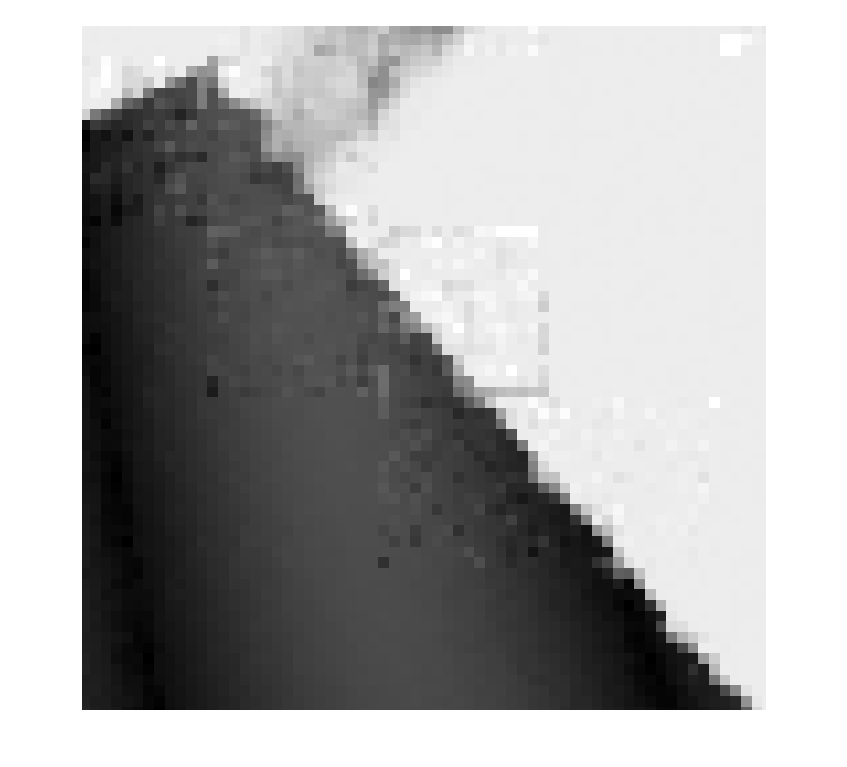
\includegraphics[width=\columnwidth]{images/boundaryArtifact_noframe.png}
  \caption{Artifacts that occur without a frame (frame size = 0). The patches are recognizable in the reconstruction}
  \label{fig:boundaryArtifacts}
\end{figure}

((( TODO: Insert plot MissingPixels vs. Accuracy )))

Use examples and illustrations to clarify ideas and results. For
example, by comparing Figure~\ref{fig:framing} and
Figure~\ref{fig:flowchart}, we can see the two different
situations where Fourier and wavelet basis perform well. 

\section{Summary}
(((( TODO ))))
  Summarise your contributions in light of the new
  results.
  

\section*{Acknowledgements}
We would like to recognize and thank the following individuals or groups for their contribution to this work:\\
Our implementation is based on the inpainting and evaluation framework provided by the course "Computer Intelligence Lab" held by Prof. Joachim Buhmann at ETH Zürich.
(((( TODO ))))


\bibliographystyle{IEEEtran}
\bibliography{biblio}

\end{document}
